%%%%%%%%%%%%%%%%%%%%%%%%%%%%%%%%%%%%%%%%%%%%%%%%%%%%%%%%%%%%%%%%%
% Contents : The first start chapter
% $Id : grisbi-manuel-start.tex, v 0.4 2002/10/27 Daniel Cartron
% $Id : grisbi-manuel-start.tex, v 0.5.0 2004/06/01 Loic Breilloux
% $Id : grisbi-manuel-start.tex, v 0.6.0 2011/11/17 Jean-Luc Duflot
% $Id : grisbi-manuel-start.tex, v 0.8.9 2012/04/27 Jean-Luc Duflot
% $Id : grisbi-manuel-start.tex, v 1.0 2014/02/12 Jean-Luc Duflot
% $Id : grisbi-manuel-start.tex, v 3.0 2024/11 Dominique Brochard
%	- comment \ifIllustration to always have pictures in manuel
%	- accounts' file to accounting's file / fichier de compteS vers fichier de comptabilité
%	- add new "start_category_select" screenshot (4/6)
%	- rewriting
%%%%%%%%%%%%%%%%%%%%%%%%%%%%%%%%%%%%%%%%%%%%%%%%%%%%%%%%%%%%%%%%%


\chapter{Premier démarrage de Grisbi\label{start}}


\section{Assistant premier démarrage\label{start-first}}


Après l'installation de Grisbi et au premier lancement du logiciel, celui-çi vous aidera avec trois assistants consécutifs:
\begin{enumerate}
	\item Le premier assistant \frquote{Bienvenue dans Grisbi !}, (qui ne s'affichera qu'une seule fois, au premier lancement), vous aide à configurer l'application. Il comprend deux étapes, dont la deuxième qui concerne la gestion du \indexword{fichier de comptes}\index{fichier de comptes} (chargement et enregistrement automatiques, chiffrement et copies de sauvegarde).

\begin{figure}[htbp]
	\begin{center}
		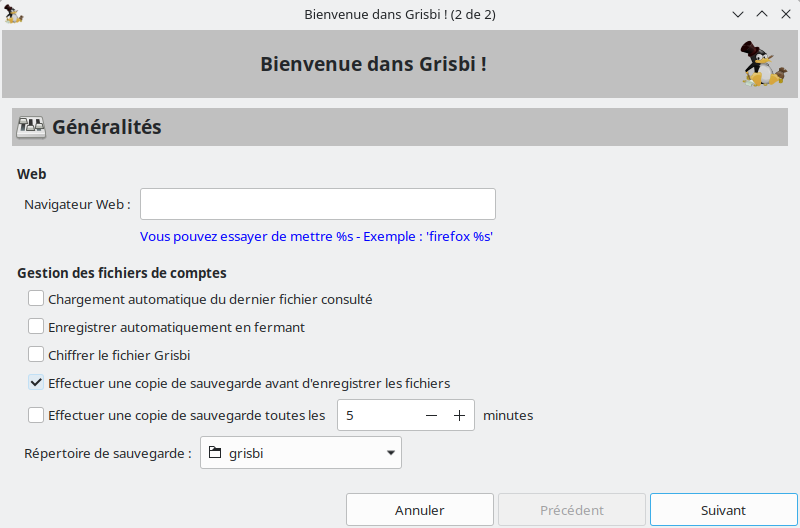
\includegraphics[width=0.9\textwidth]{image/screenshot/start_first_launch}
	\end{center}
	\caption{Configuration initiale du fichier de comptes.}
	\label{start_first_launch}
\end{figure}

Il est conseillé de cocher les options:
	\begin{itemize}
		\item Chargement automatique du dernier fichier consulté;
		\item Enregistrer automatiquement en fermant;
		\item Effectuer une copie de sauvegarde avant d'enregistrer les fichiers (coché par défaut).
	\end{itemize}
\end{enumerate}

\minisec{\textcolor{red}{\strong{Attention:}}}
Les développeurs de Grisbi vous recommandent de ne pas utiliser l'option \menu{Chiffrer le fichier Grisbi} pour les raisons suivantes: 
	\begin{itemize}
		\item il n’existe aucune méthode pour récupérer un fichier chiffré dont on a perdu le mot de passe;
		\item Pour une raison inconnue, l’utilisation de cette option sous Windows peut rendre le fichier de comptes totalement inutilisable.
	\end{itemize}  
Néanmoins, si vous l'utilisez, il est recommandé de faire régulièrement des sauvegardes du fichier non chiffré.

\vspacepdf{3mm}
\begin{enumerate}[resume]
	\item Le deuxième assistant \frquote{Bienvenue dans Grisbi !} (ou plus tard \frquote{Aide à la création d'un nouveau fichier de comptes}), qui suit automatiquement le premier, comprend six étapes qui vous aiderons à la création du \indexword{fichier de comptes}\index{fichier de comptes}. 
	\item Puis vient automatiquement le troisième assistant \frquote{Créer un nouveau compte} qui permet de créer le premier compte et qui est décrit en détail dans la section \ref{start-newfile} ci-dessous.
\end{enumerate}
À tout moment vous pouvez sortir de n'importe quel assistant par le bouton \menu{Annuler}.

Si vous ne voulez pas utiliser l'assistant premier démarrage, vous pouvez à la
place utiliser un fichier exemple (voir la section \ref{start-example} ci-dessous).


\section{Fichier exemple\label{start-example}}


Si vous voulez utiliser Grisbi immédiatement sans être obligé de rentrer tout un tas d'opérations, par exemple pour vous faire une idée des possibilités de ce logiciel, vous pouvez télécharger le fichier \file{Example\_3.0-fr.gsb} sur le site de \lang{Sourceforge.net}\footnote{\urlSourceForgeDocumentation{}} dans le dossier \frquote{\textsf{examples}}.

% espace avant Attention ou Note  :  5mm
\vspacepdf{5mm}
\textbf{Note}: dans ce fichier exemple, les noms des tiers sont de pure invention; seul un hasard indépendant de notre volonté peut avoir fait que ce soit celui d'une personne ou d'une entité existante.


\section{Création d'un nouveau fichier de comptes\label{start-newfile}}


La première fois que vous utiliserez Grisbi, vous devrez d'abord créer un \indexword{fichier
de comptes}\index{fichier de comptes} qui contiendra votre comptabilité. L'\gls{extension} de ce fichier sera \file{.gsb} et son nom \file{nom-de-votre-fichier.gsb}. 

Immédiatement après, il vous faudra créer au minimum un compte (bancaire, de caisse, de passif ou d'actif, décrits au chapitre \vref{accounts} \menu{Gestion des comptes}), et par la suite quelques autres comptes (comptes courants, d'épargne, de crédit, éventuellement un compte d'espèces et quelques comptes de transition) qui contiendront leurs opérations respectives. 

Pour une gestion familiale, vous n'aurez normalement qu'un seul fichier de comptes, car cela permet tous les échanges entre vos différents comptes. Si vous gérez une association, ou une autre famille sans rapport comptable avec la première, vous créerez un autre fichier de comptes, qui portera un autre nom \file{nom-de-votre-deuxième-fichier.gsb}. Ainsi les \indexword{entités comptables}\index{entité comptable} resteront bien séparées.

Autrement dit, l’ensemble des comptes de votre foyer est enregistré dans un fichier de comptes,
et l’ensemble des comptes de votre association l’est dans un autre fichier de comptes.

% espace pour changement de thème
\vspacepdf{5mm}
%Le déroulement général de la procédure de création d'un fichier de comptes est le suivant: cliquez sur le menu \menu{Fichier > Nouveau fichier de comptes}; l'assistant \frquote{Aide à la création d'un nouveau fichier de comptes}, qui comprend six étapes, s'ouvre. À la sixième étape, l'assistant vous propose:

%\begin{itemize}
%	\item soit de créer un nouveau compte vide, et il enchaîne sur l'assistant \frquote{Créer un nouveau compte}, qui comprend lui-même quatre étapes, pour créer le premier compte (car il est indispensable de disposer d'au moins un compte);
%	\item soit d'utiliser des données déjà existantes, et il enchaîne alors sur l'assistant \frquote{Importation des opérations par Grisbi}, qui comprend aussi quatre étapes, pour importer des opérations de comptes existants.
%\end{itemize}

% espace pour changement de thème
%\vspacepdf{5mm}
Pour créer votre fichier de comptes, cliquez sur le menu \menu{Fichier > Nouveau fichier de comptes} ou sur le pavé Nouveau\refimage{start_grisbi}, et la procédure se déroulera en six étapes détaillées comme suit:

\begin{enumerate}
	\item Fenêtre d'accueil (étape 1/6): validez par le bouton \menu{Suivant}:
	\item Configuration
 générale (étape 2/6)\refimage{start_file_create}:

\begin{figure}[htbp]
\begin{center}
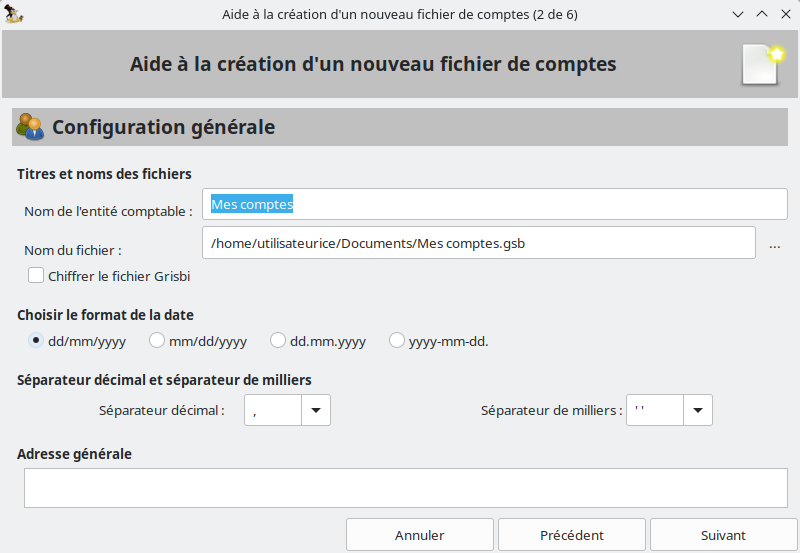
\includegraphics[width=0.9\textwidth]{image/screenshot/start_file_create}
\end{center}
\caption{Configuration générale du fichier de comptes}
\label{start_file_create}
\end{figure}
		
		\begin{enumerate}
		 	\item choisissez le nom de l'entité comptable dont vous gérez la comptabilité, par exemple \frquote{Ma comptabilité}, qui pourra être choisi comme titre de la page d'accueil de l'application Grisbi,
			\item saisissez le nom du fichier de comptes avec son arborescence complète; Grisbi vous propose par défaut le même nom que celui de l'entité comptable, mais vous pouvez le modifier,
			\item cochez la case \menu{Chiffrer le fichier Grisbi} si vous voulez \gls{chiffrer} le fichier de comptes,
			
			%\vspacepdf{1mm}
			%\textcolor{red}{\strong{Attention}}: si vous cochez l'option \menu{Chiffrer le fichier Grisbi}, la perte du mot de passe rendra votre fichier inaccessible.
			%\vspacepdf{2mm}
		\end{enumerate}

\minisec{\textcolor{red}{\strong{Attention:}}}
%\textcolor{red}{\strong{\textsf{Attention:}}}\newline
Les développeurs de Grisbi vous recommandent de ne pas utiliser l'option \menu{Chiffrer le fichier Grisbi} pour les raisons suivantes: 
\begin{itemize}
	\item il n’existe aucune méthode pour récupérer un fichier chiffré dont on a perdu le mot de passe;
	\item Pour une raison inconnue, l’utilisation de cette option sous Windows peut rendre le fichier de comptes totalement inutilisable.
\end{itemize}  
Néanmoins, si vous l'utilisez, il est recommandé de faire régulièrement des sauvegardes du fichier non chiffré.			

		\begin{enumerate}[resume]		% to resume \end{enumerate} above \minisec
			\item sélectionnez le \indexword{format de la date}\index{format de date} avec l'un des quatre boutons:
			%\begin{addmargin}{-0.2cm}
				\begin{itemize}	
				\item[\textopenbullet] "dd/mm/yyyy" pour "jour/mois/année",
				\item[\textopenbullet] "mm/dd/yyyy" pour "mois/jour/année",
				\item[\textopenbullet] "dd.mm.yyyy" pour "jour.mois.année",
				\item[\textopenbullet] "yyyy-mm-dd" pour "année-mois-jour",
				\end{itemize}
			%\end{addmargin}
			\item choisissez le \indexword{séparateur}\index{séparateur} décimal et celui des milliers dans les listes déroulantes,
			\item renseignez l'adresse (facultatif),
			\item validez par le bouton \menu{Suivant};
		\end{enumerate}
		
	\item Sélection de la \indexword{devise}\index{devise} de base (étape 3/6):
		\begin{enumerate} 
		 	\item cliquez sur la devise choisie dans la liste,
			\item cochez la case \menu{Afficher les devises obsolètes} si vous voulez aussi afficher d'anciennes devises,
			\item validez par le bouton \menu{Suivant};
		\end{enumerate}

	\item sélection des \indexword{types de catégories}\index{catégories!types} utilisées (étape 4/6)\refimage{start_category_select}:
	
	\begin{figure}[htbp]
	\begin{center}
		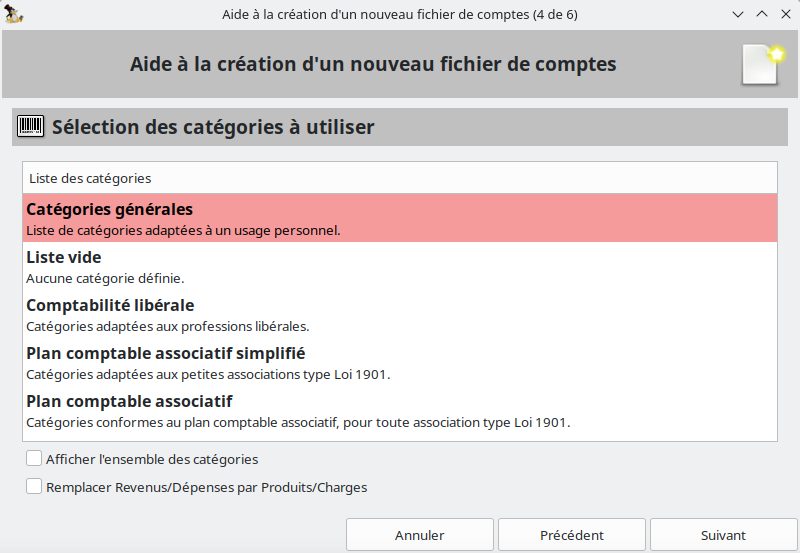
\includegraphics[width=0.9\textwidth]{image/screenshot/start_category_select}
	\end{center}
	\caption{Sélection des catégories à utiliser}
	\label{start_category_select}
	\end{figure}
		
		\begin{enumerate} 
		 	\item cliquez sur la catégorie choisie dans la liste;
%		 	\begin{itemize}
%		 		\item\menu{Catégories générales},
%		 		\item \menu{Liste vide},
%		 		\item\menu{Comptabilité libérale},
%		 		\item\menu{Plan comptable associatif simplifié}
%		 		\item\menu{Plan comptable associatif},
%		 	\end{itemize}
			\item cochez la case \menu{Afficher l'ensemble des catégories} si vous voulez aussi afficher d'autres catégories libellées en anglais,
			\item validez par le bouton \menu{Suivant};
		\end{enumerate}		

	\item Définissez les \indexword{banques}\index{banques!définition} détenant vos comptes (étape 5/6):
		\begin{enumerate} 
		 	\item cliquez sur \menu{Ajouter} pour définir une banque; renseignez les détails de la banque (nom, code banque, etc.), puis validez par le bouton \menu{Ajouter} pour valider la banque,
			\item sélectionnez une banque dans la liste et validez par le bouton \menu{Enlever} pour supprimer une banque, puis confirmez dans la fenêtre qui s'ouvre,
			\item répétez les actions a et b autant de fois que nécessaire,
			\item validez par le bouton \menu{Suivant} pour passer à l'étape suivante, \menu{Création d'un nouveau compte};
		\end{enumerate}		 	

	\item Configuration terminée (étape 6/6)\refimage{start_account_choice}:\par
	La configuration du fichier de comptes est terminée, et la fenêtre ci-dessous vous propose de choisir l'une des deux méthodes de création de votre premier compte:

\vspace{2mm}

\begin{figure}[htbp]
\begin{center}
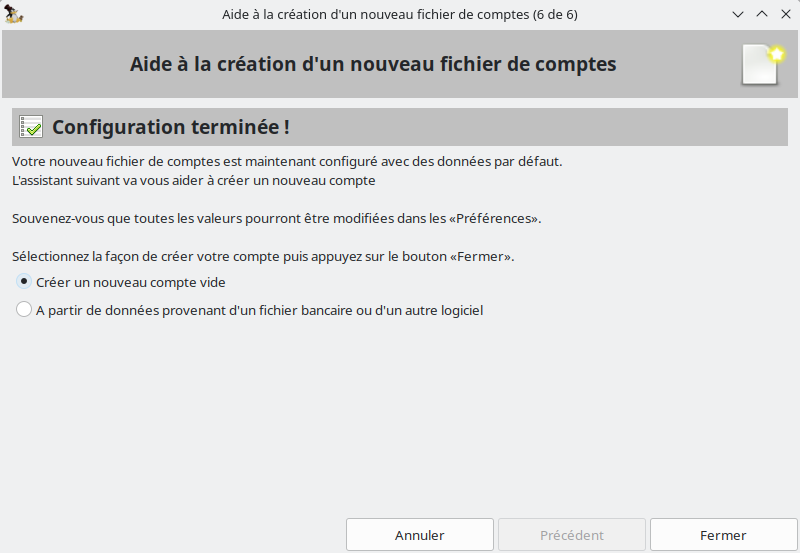
\includegraphics[width=0.9\textwidth]{image/screenshot/start_account_choice}
\end{center}
\caption{Choix du premier compte}
\label{start_account_choice}
\end{figure}

		\begin{itemize}
			\item[\textopenbullet] \menu{Créer un nouveau compte vide}: si vous cochez cette ligne, puis si vous validez par le bouton \menu{Fermer}, cette fenêtre se ferme et l'assistant \frquote{Créer un nouveau compte} démarre. Reportez-vous à la section \vref{accounts-new}%8.4
			, \menu{Création d'un nouveau compte}, qui décrit entièrement cette procédure, puis revenez à cette page;

			\item[\textopenbullet] \menu{À partir de données provenant d'un fichier bancaire ou d'un autre logiciel}: si vous cochez cette ligne, puis si vous validez par le bouton \menu{Fermer}, cette fenêtre se ferme et l'assistant \frquote{Importation des opérations par Grisbi}, permettant l'importation de données d'un fichier de comptes, démarre. Reportez-vous à la section \vref{move-import-importinit}%6.1.2
			, \menu{Import de fichiers de compte d'un autre logiciel dans Grisbi}, qui décrit entièrement cette procédure, puis revenez à cette page.
		\end{itemize}
\end{enumerate}

% étiquette du paragraphe suivant, pour que les liens hypertexte dans account.tex et QIF.tex  arrivent bien dessus
\label{start-newfile-end}

\textit{\textbf{D'une manière ou d'une autre}}, vous venez donc de créer votre fichier de comptes, ainsi que le premier compte de ce fichier. 

%espace pour changement de thème
\vspacepdf{5mm}
Si vous voulez créer maintenant d'autres comptes, sélectionnez le menu \menu{Édition - Nouveau compte} pour créer un autre compte (voir la section \vref{accounts-new}, \menu{Création d'un nouveau compte}).

%espace pour changement de thème
\vspacepdf{5mm}
Sinon, vous pouvez commencer à utiliser le compte que vous venez de créer ou celui dont vous venez d'importer les données.

% espace avant Attention ou Note  : 5 mm
%\vspacepdf{5mm}
\minisec{\textcolor{red}{\strong{Attention:}}}
D'une manière générale, il est déconseillé d'avoir des accents ou des espaces dans les noms des répertoires et fichiers utilisés par Grisbi. Si c'est le cas, renommez-les maintenant. Par exemple, les espaces peuvent être remplacées par des tirets bas (\_).

% saut de page pour titre solidaire
%\newpage


\section{Enregistrement de votre fichier de comptes\label{start-save}}


Vos opérations ne sont pas écrites au fur et à mesure de leur saisie comme elles peuvent l'être dans d'autres logiciels; vous devez donc enregistrer votre fichier de comptes avant de quitter. N'ayez crainte, Grisbi vous prévient si vous ne l'avez pas fait. 

Vous pouvez configurer les options d'enregistrement du fichier de comptes dans le menu \menu{Édition - Préférences}, voir le paragraphe \vref{setup-general-files-manage}, \menu{Gestion des fichiers de comptes}.


\section{Import à partir d'un autre logiciel de comptabilité personnelle}

Voir la section \vref{move-import-importinit} pour importer des fichiers de compte d'un autre logiciel dans Grisbi. Pour le moment, Grisbi supporte les formats \gls{Gnucash}, \gls{OFX}, \GLS{CSV} et \GLS{QIF}.


